%% LaTeX2e class for student theses
%% thesis.tex
%% 
%% Karlsruhe Institute of Technology
%% Institute for Program Structures and Data Organization
%% Chair for Software Design and Quality (SDQ)
%%
%% Dr.-Ing. Erik Burger
%% burger@kit.edu
%%
%% See https://sdq.kastel.kit.edu/wiki/Dokumentvorlagen
%%
%% Version 1.3.6, 2022-09-28

%% Available page modes: oneside, twoside
%% Available languages: english, ngerman
%% Available modes: draft, final (see README)
\documentclass[oneside, english, final]{sdqthesis}

%% ---------------------------------
%% | Information about the thesis  |
%% ---------------------------------

%% Name of the author
\author{Wenzhe Vincent Cui}

%% Title (and possibly subtitle) of the thesis
\title{Confidential Computing in Distributed Systems}

%% Type of the thesis 
\thesistype{Bachelor's Thesis}

%% Change the institute here, ``KASTEL'' is default
\myinstitute{SCC -- Steinbuch Centre for Computing}

%% You can put a logo in the ``logos'' directory and include it here
%% instead of the SDQ logo
% \grouplogo{myfile}
%% Alternatively, you can disable the group logo
% \nogrouplogo

%% The reviewers are the professors that grade your thesis
\reviewerone{Prof. A}
\reviewertwo{Prof. B}

%% The advisors are PhDs or Postdocs
\advisorone{M.Sc. C}
%% The second advisor can be omitted
\advisortwo{M.Sc. D}

%% Please enter the start end end time of your thesis
\editingtime{30. November 2022}{30. March 2023}

\settitle

%% --------------------------------
%% | Bibliography                 |
%% --------------------------------

%% Use biber instead of BibTeX, see README
\usepackage[citestyle=numeric,style=numeric,backend=biber]{biblatex}
\addbibresource{thesis.bib}

%% Todos
\usepackage[obeyDraft]{todonotes}

%% ====================================
%% ====================================
%% ||                                ||
%% || Beginning of the main document ||
%% ||                                ||
%% ====================================
%% ====================================
\begin{document}

%% Set PDF metadata
\setpdf

%% Set the title
\maketitle

%% The Preamble begins here
\frontmatter

%% LaTeX2e class for student theses: Declaration of independent work
%% sections/declaration.tex
%% 
%% Karlsruhe Institute of Technology
%% Institute for Program Structures and Data Organization
%% Chair for Software Design and Quality (SDQ)
%%
%% Dr.-Ing. Erik Burger
%% burger@kit.edu
%%
%% Version 1.3.6, 2022-09-28

\thispagestyle{empty}
\null\vfill
\noindent\hbox to \textwidth{\hrulefill} 
\iflanguage{english}{I declare that I have developed and written the enclosed
thesis completely by myself. I have submitted neither parts of nor the complete 
thesis as an examination elsewhere. I have not used any other than the aids that
I have mentioned. I have marked all parts of the thesis that I have included from 
referenced literature, either in their original wording or paraphrasing their
contents. This also applies to figures, sketches, images and similar depictions,
as well as sources from the internet.}%
{Ich versichere hiermit, dass ich die vorliegende Arbeit selbstständig verfasst,
und weder ganz oder in Teilen als Prüfungsleistung vorgelegt und keine anderen
als die angegebenen Hilfsmittel benutzt habe. Sämtliche Stellen der Arbeit, die
benutzten Werken im Wortlaut oder dem Sinn nach entnommen sind, habe ich durch
Quellenangaben kenntlich gemacht. Dies gilt auch für Zeichnungen, Skizzen,
bildliche Darstellungen und dergleichen sowie für Quellen aus dem Internet. }
 
 
%% ---------------------------------------------
%% | Replace PLACE and DATE with actual values |
%% ---------------------------------------------
\textbf{PLACE, DATE}
\vspace{1.5cm}
 
\dotfill\hspace*{8.0cm}\\
\hspace*{2cm}(\theauthor) 
\cleardoublepage

\setcounter{page}{1}
\pagenumbering{roman}

%% ----------------
%% |   Abstract   |
%% ----------------

\listoftodos
 
%% For theses written in English, an abstract both in English
%% and German is mandatory.
%%
%% For theses written in German, a German abstract is sufficient.
%%
%% The text is included from the following files:
%% - sections/abstract

%\includeabstract
%% LaTeX2e class for student theses
%% sections/abstract_en.tex
%% 
%% Karlsruhe Institute of Technology
%% Institute for Program Structures and Data Organization
%% Chair for Software Design and Quality (SDQ)
%%
%% Dr.-Ing. Erik Burger
%% burger@kit.edu
%%
%% Version 1.3.6, 2022-09-28

\Abstract

In the current computing landscape distributed computing systems, largely based
on Grid and Cloud computing, have become the main ways of sharing infrastructure
resources, such as compute, storage, and network resources, while also providing
services that ease the development and orchestration of applications on said
resources. On the one hand, the usage of these resources and service come with
benefits such as higher availability, reducing complexity of applications, and
cost-efficiency, on the other hand, traditionally these benefits come with the
cost of fully trusting the provider of the resources and services with
potentially confidential data. Nevertheless, as consumer and government demands
for data privacy increase (e.g., GDPR coming into effect in the EU in 2018), the
distributed computing model must adapt to meet the increasingly strict trust
requirements. The advent of confidential computing enables a new distributed
computing model where the provider of infrastructure resources becomes untrusted
by providing hardware-based trusted execution environments (TEEs). This thesis
researches the current state of trusted execution environment technologies,
remote attestation procedures that allow tenants to verify the trustworthiness
of TEEs, and introduces a new \textit{trusted distributed computing model} that
integrates these two concepts into the traditional distributed computing model
in order to remove the provider of the distributed computing system from the
list of trusted parties.


%% ------------------------
%% |   Table of Contents  |
%% ------------------------
\tableofcontents

\listoffigures
\listoftables

%% -----------------
%% |   Main part   |
%% -----------------

\mainmatter

\chapter{Introduction}
%% LaTeX2e class for student theses
%% sections/content.tex
%% 
%% Karlsruhe Institute of Technology
%% Institute for Program Structures and Data Organization
%% Chair for Software Design and Quality (SDQ)
%%
%% Dr.-Ing. Erik Burger
%% burger@kit.edu
%%
%% Version 1.3.6, 2022-09-28

\chapter{Introduction}
\label{ch:Introduction}

\section{Background}
\label{sec:background}

\section{Motivation}
\label{sec:motivation}

\section{Research Methodology}
\label{sec:research-methodology}


\chapter{Background}
\section{Cryptographic Concepts}
\label{sec:cryptographic-concepts}

Cryptography is the practice of protecting data by transforming it into a format
that is unreadable by an unauthorized party. In this background section we will
have a look at the basics of symmetric cryptography, asymmetric cryptography,
and key agreement protocols.

\subsection{Symmetric and Asymmetric Cryptography}
\label{sec:symmetric-asymmetric-cryptography}

Symmetric cryptography, also known as secret-key cryptography, is a method of
encryption where the same key is used for both encryption and decryption. This
means that both the sender and receiver must have the same key to encrypt and
decrypt messages. In symmetric cryptography, the key is kept secret and secure
to prevent unauthorized access. The most common symmetric encryption algorithms
are Advanced Encryption Standard (AES) and Data Encryption Standard (DES).

The main benefit of symmetric cryptography is its performance. Since the same
key is used for encryption and decryption, it is a fast and efficient process.
However, one of the major drawbacks of symmetric cryptography is the issue of
key management. Managing and distributing keys to entities and components that
require access to encrypted data is a challenging task. Furthermore, if a key is
compromised, all data encrypted with that key can be easily decrypted.

Asymmetric cryptography, also known as public-key cryptography, is a method of
encryption where two different keys are used for encryption and decryption.
These keys are mathematically related, but they cannot be derived from each
other. One key is kept private, and the other key is made public. The private
key is used for decryption, while the public key is used for encryption. The
most common asymmetric encryption algorithms are RSA and Elliptic Curve
Cryptography (ECC).

One of the significant benefits of asymmetric cryptography is that it eliminates
the need for key management. Each user or system can have a unique pair of
public and private keys, and the public key can be shared with anyone. The
private key, on the other hand, is kept secure and confidential. Asymmetric
cryptography is slower than symmetric cryptography due to the complexity of the
mathematical algorithms involved. However, it is more secure since even if the
public key is compromised, the private key cannot be derived from it.

Digital signature is a widely used application of asymmetric cryptography. A
digital signature is a cryptographic primitive that is used to verify the
integrity and authenticity of a data. The process of digital signature involves
two steps: signing and verification. To sign data, the owner of the data uses
their private key to generate a unique digital signature. When the owner sends
the data together with the signature to another party, the receiver can use the
owner's public key to verify the signature's authenticity and the data's
integrity. If the verification of the digital was successful, the receiver can
be confident that the data was sent by the owner has not been modified during
transit.

\subsection{Key Agreement}
\label{sec:key-agreement}

Key agreement is a crucial component of secure communication. It involves two
parties agreeing on a secret key (symmetric cryptography) that can be used for
encryption and decryption of messages. One of the most popular key agreement
protocols is the Diffie-Hellman protocol.

The Diffie-Hellman protocol is a key agreement protocol that utilizes asymmetric
cryptography in order to allow two parties to agree on a mutual secret key over
an insecure channel. A simplified overview of the process is as follows (with
parties Alice and Bob):

\begin{enumerate}
  \item Both parties establish shared parameters: a prime number $p$ and
        generator $g$.
  \item Each party generates a random number ($A$ for Alice and $B$ for Bob) and
        computes a publicly known number $pub_A = g^A \mod p$ and $pub_B = g^B
          \mod p$ respectively.
  \item Both parties exchange their public number $pub_A$ and $pub_B$.
  \item Both parties compute the shared secret key $K = (pub_A)^B = (pub_B)^A =
          g^{AB} \mod p$
  \item The secret key $K$ can then be used to encrypt and decrypt messages send
        between both parties, establishing a secure communication channel over
        an insecure channel.
\end{enumerate}

Even though attackers might gain knowledge about $p$, $g$, $pub_A$, and $pub_B$
by listening to the insecure channel, they can not derive the secret key $K$
from the publicly known numbers. If we assume that the prime number $p$ and
generator $g$ are already specified in a specific protocol or have been
pre-established, there are exactly two messages that need to be exchanged
between Alice and Bob. For example, if Alice is the initiator of the
communication, Alice starts by sending $pub_A$ upon which Bob responds with
$pub_B$. After exchanging those two messages, Alice and Bob can already derive
the shared secret key $K$.

However, an attacker might perform a man-in-the-middle attack, where the
attacker intercepts the key agreement process and establishes shared secrets
with both Alice and Bob. If Alice sends Bob an encrypted message, the attacker
decrypts the message using the shared secret key with Alice, gains access to the
plain text content of the message, encrypts the message using the shared secret
with Bob, and finally relays the message to Bob.

Furthermore, the attacker can even impersonate either party in the
communication. For example, Bob thinks that the secret key he/she established
with the attacker is only known by Bob and Alice. Therefore, Bob assumes that
messages encrypted with this secret key and send to Bob by the attacker, are
sent by Alice.

In order to mitigate man-in-the-middle attacks, either Alice or Bob has to
authenticate the other party. This can be achieved using asymmetric
cryptographic keys. For example, Bob uses his own private key to sign the
message that includes $pub_B$ and is sent to Alice. Alice then uses Bob's public
key in order to verify that the message is indeed sent by Bob. The public keys
can be securely exchanged between Alice and Bob by facilitating a Public Key
Infrastructure (PKI). However, this thesis will not further go into detail about
PKIs.


\chapter{Technical Research}
\label{ch:technical-research}
\section{Traditional Distributed Computing Model}
\label{sec:traditional-distributed-computing}

Distributed computing systems are inherently distributed systems, which means
they share the fundamental characteristics and goals, defined by
\citeauthor{tannenbaum2017} \cite{tannenbaum2017} as resource sharing,
transparent distribution, openness, and scalability. Distributed computing
facilitate distributed system principles in order to group a set of resources
(possibly at a geographical distance) and provide tenants a single, coherent
view of these resources. In general distributed computing systems allow users to
share, manage the access to, and use compute, storage, and network resources.

In the following two sections we will look at two major distributed computing
concepts, Grid and Cloud computing.

\subsection{Grid Computing}

The Grid Computing model focuses on sharing widely distributed compute resources
in order provide problem-solving environments and enable collaboration for a set
of individuals or institutions, so-called virtual organizations. It provides
basic mechanisms, in the form of network protocols and interfaces. These
protocols and interfaces offer means of discovering, managing the access to, and
using remote resources. Because those resources are not subject to centralized
control, these protocols and interfaces have to be standardized and open to
enable interoperability \cite{foster2001grid}.

The hourglass model facilitated by the internet protocol stack can also be found
in the Grid computing architecture. While the base of the hourglass provides
various fundamental behaviors, the neck defines a small set of abstractions,
allowing a diverse set of high-level behaviors to be built on top. The four
layers of the Grid computing model are as follows:

\begin{figure}[H]
  \centering
  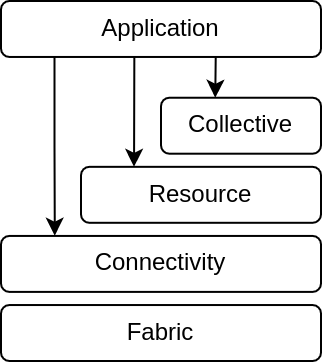
\includegraphics[width=0.3\linewidth]{resources/grid-architecture.drawio.png}
  \caption[The layered Grid architecture.]{
    The layered Grid architecture.\\
    Source: \citeauthor{foster2001grid} \cite{foster2001grid}
  }
  \label{fig:grid-architecture}
\end{figure}

\begin{description}
  \item[Fabric Layer]
    The Fabric layer provides the resources which are shared by Grid protocols
    and offers local, resource-specific operations that occur on specific
    resources as a result of sharing operations at higher levels. This should at
    least provide resource enquiry mechanisms, enabling the discovery of their
    structure, state and capabilities, and resource management mechanisms,
    providing control over them.
  \item[Connectivity]
    This layer specifies core communication and authentication protocols,
    enabling the exchange of data between Fabric layer resources and providing
    secure mechanisms for verifying the identity of users and resources.
    Communication usually requires transport, routing, and naming protocols.
  \item[Resource]
    On top of the Connectivity layer the Resource layer defines protocols
    providing secure negotiation, initiation, monitoring, control, accounting,
    and payment mechanisms for individual resources. It utilizes Fabric layer
    functions in order to access and control local resources. These protocols
    are focused on a single resource, implying that they ignore issues of global
    state and atomic actions across distributed collections.
  \item[Collective]
    While the Resource layer is concerned with the interactions of a single
    resource, the Collective layer focuses on the interaction of a collection of
    resources. Being the top and building on the neck (Connectivity and Resource
    layer) of the hourglass allows this layer to provide a wide variety of
    behaviors, such as discovering, co-allocation, scheduling, brokering,
    monitoring, and replication of resources.
  \item[Applications]
    The final layer of the Grid architecture is the collection of user
    applications. These applications implement specific business logics by
    utilizing resources and services of the previous layers.
\end{description}

\subsection{Cloud Computing}

Cloud Computing systems usually have a centralized control and facilitate both
open and proprietary protocols and interfaces in order to provide on-demand
self-service, broad network access, resource pooling, rapid elasticity, and
measured services. \citetitle{mell2011} \cite{mell2011} defines three distinct
service models of cloud computing:

\begin{description}
  \item[Infrastructure as a Service (IaaS)]
    In an IaaS service model the managed resources are fundamental computing
    resources. This includes -- physical or virtual -- machines, storage, and
    networks. The consumer does not manage or control the underlying
    infrastructure but can deploy and run arbitrary software, including
    operating systems, onto the provided infrastructure.

  \item[Platform as a Service (PaaS)]
    The PaaS service model adds another layer of abstraction on top of the IaaS
    service model. Consumers can deploy and run applications on a provided
    platform that supports a set of programming languages, libraries, services,
    and tools. So the managed resources in a PaaS service model are
    applications. The consumer does not manage or control the underlying
    infrastructure, and additionally has no control over the operating system.

  \item[Software as a Service (SaaS)]
    In this model the managed resources are applications. But in comparison to
    the PaaS model the consumer is not able to run arbitrary applications, but
    only a provider specific selection of applications. The customer does not
    manage or control the underlying infrastructure, operating system, or even
    the application.
\end{description}

These service models provide tenants with resources that applications run on and
services that support the development and deployment of these applications.

\subsection{Trust Model}

There are three roles that are present in the traditional distributed computing
model.

\begin{description}
  \item[Service Provider]
    In general a service provider is an entity or organizational unit that
    provides services to other entities or organizational units. In the
    distributed computing context service providers provide application owners
    and data owners with infrastructure resources and/or platform services.

  \item[Application Owner]
    Application owners manage applications that operate on data owned by the
    data owner. This does not imply that the application owner develops
    applications. Applications can be developed and provided by separate
    entities.

  \item[Data Owner]
    Data owners are in the possession of data that used, and/or manipulated by
    an application. They are concerned about the confidentiality of their data.
    If there are multiple data owners there may be mutual distrust between the
    data owners.
\end{description}

This trust model needs to be applied from the perspective of the data owners and
is tied to a set of data. For example, in a Grid environment, there are three
virtual organizations $A$, $B$, and $C$, all sharing resources and services.
Assuming that virtual organization $A$ owns a dataset $D$, but all of $A$'s
resources are currently occupied. Therefore, $A$ wants to use resources from
virtual organization $B$ in order to run an application on dataset $D$. In this
context, while all virtual organizations share resources, only $B$ takes on the
role of a service provider, because $A$ does not share resources used for this
specific context and $C$ is not involved at all. Because $A$ manages the
application and owns the dataset $D$, $A$ takes on the role of application owner
and data owner in this example.

Traditionally, the data owner trusts both the application owner and the service
provider. Therefore, both roles can be taken on by the same party.

\subsection{Architectural Overview}

\begin{figure}[H]
  \centering
  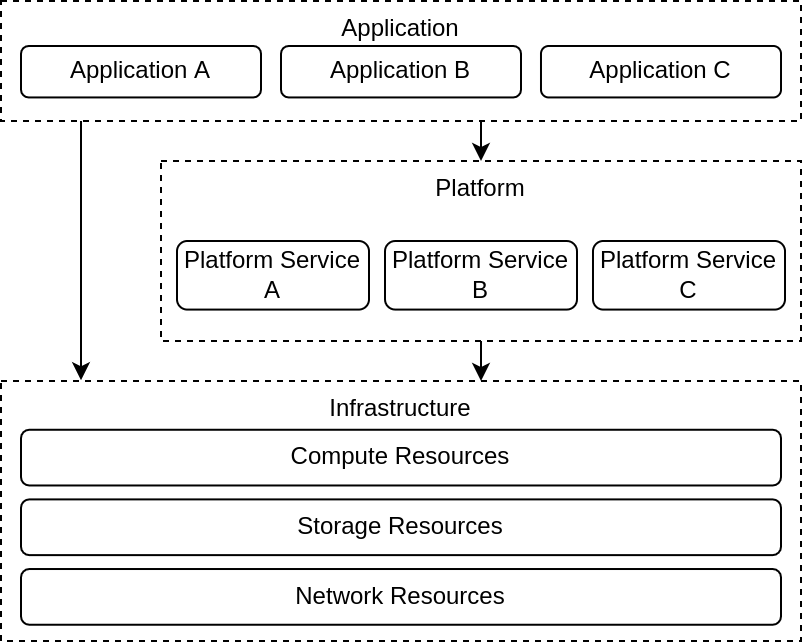
\includegraphics[width=0.7\linewidth]{resources/distributed-computing-overview.drawio.png}
  \caption{Layered model of a distributed computing system.}
\end{figure}

This section defines a generalized architecture of the distributed computing
model, which consists of three layers.

\begin{description}
  \item[Infrastructure]
    This layer provides fundamental resources, such as compute, network, and
    storage resources. This commonly includes physical or virtual machines
    (compute resource), layer two or three networks connecting machines (network
    resource), and network attached storage (storage resource).

    In the Cloud model this corresponds to the IaaS service model and in the
    Grid architecture it is represented by the Fabric layer.
  \item[Platform]
    The Platform layer sits between the Infrastructure and Application layer. It
    provides a set of services and tools that support application owners to run
    applications in a distributed computing environment and manage the
    underlying infrastructure resources required for the application to run. The
    platform layer abstract the complexity of the underlying infrastructure by
    providing services to manage, access, and utilize needed resources. These
    services are all operated and provided by the service provider.

    This layer matches the Cloud's PaaS and SaaS service model and is
    represented by the collection of the Resource, Connection, and Collective
    layer in the Grid architecture.
  \item[Application]
    The final layer is the collection of applications and services managed by
    application owners.
\end{description}

In the following figures components of the Infrastructure layer are marked in
blue, Platform layer in red, and Application layer in green.

\subsubsection{Infrastructure Layer}

\begin{figure}[H]
  \centering
  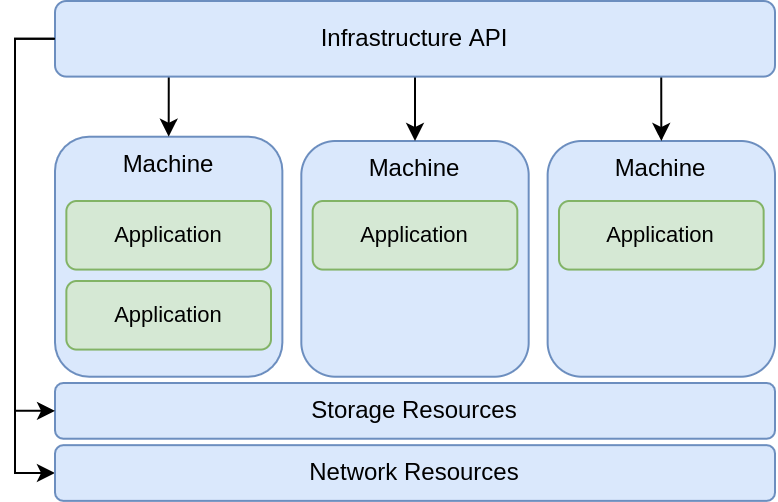
\includegraphics[width=0.7\linewidth]{resources/distributed-computing-infrastructure-example.drawio.png}
  \caption{Overview of the Infrastructure layer in the traditional distributed computing model.}
  \label{fig:traditional-infrastructure-overview}
\end{figure}

Typically, computing resources provided by the Infrastructure layer are in the
form of physical or virtual machines. These machines combine CPUs, memory, and
peripheral devices. On the other hand, storage and network resources can be
provided in various forms, such as block-level, file-level, and object-level
storage, and layer two and three networks. In order to keep this model abstract,
we will not make any assumptions about specifics of the storage and network
resources. This model will assume the presence of an application programming
interface (API), that can be used to implement a user interface. While various
kinds of user interfaces can be provided to tenants, such as websites, web
portals, terminal user interfaces (TUIs), graphical user interfaces (GUIs),
software development kits (SDKs), and libraries, these user interfaces typically
facilitate an API that exposes resource management actions.

As outlined before, there are two types of resources in the Infrastructure
layer: physical and virtual. Physical Infrastructure layer resources protection
is implemented by the service providers. For example by securing the physical
location of the hardware and utilizing application transparent encryption.
Virtual infrastructure is protected by the isolation that virtualization systems
provide. This requires a correctly configured and actively patched
virtualization system, as misconfiguration can lead to breaking the isolation
guarantees, and not patching virtualization systems allows attackers to exploit
vulnerabilities in those implementations. For example hypervisors are large
pieces of software that require complex configuration, and over the years
numerous vulnerabilities have been found in commonly used hypervisors
\cite{perezbotero2013hypervisorvulnerabilities,
  reuben2007surveyvirtualmachinesecurity}. These virtualization systems are
generally managed and controlled by the service provider. Therefore, protection
of infrastructure layer resources, regardless of whether the resources are
physical or virtual, is entrusted to the service provider.


\subsubsection{Platform Layer}

The platform layer offers various kinds of services. Commonly found services
are:

\begin{description}
  \item[Resource management]
    Management of compute and storage resources. This could include the ability
    to (co-)allocate and release resources in order to dynamically scale
    depending on the current needs, and monitor resource usage.
  \item[Authentication and authorization]
    Providing ways to verify the identity of a user or process and define and
    enforce policies governing the access to infrastructure resources and
    applications.
  \item[Messaging and communication]
    While the infrastructure provides basic infrastructure for communication by
    providing network resources, the platform layer often provides higher level
    communication such as inter-process communication, message passing, and
    event notifications.
  \item[Data management]
    Providing means for storing and accessing data by managing storage resources
    of the Infrastructure layer. Often also provides caching, replication,
    synchronization services in order to maximize availability, integrity, and
    performance.
  \item[Service discovery and load balancing]
    Exposing applications as network services to other applications and
    distributing traffic to multiple instance of an application.
  \item[Monitoring and logging]
    Support the monitoring of applications for failures and performance issues
    and aggregate logs of applications for debugging and auditing purposes.
  \item[Collaboration frameworks]
    Provide problem-solving environments that manage multistep, asynchronous,
    multi-component workflows.
  \item[Application deployment]
    Decrease the burden of deploying applications, providing mechanisms to
    deploy and configure applications in execution environments.
  \item[Key Management]
    A Key Management Service (KMS) manage cryptographic keys used to encrypt and
    decrypt confidential data. These services typically provide mechanisms for
    generating, storing, and providing keys to other applications and services.
\end{description}

While these services implement various types of behaviors, they can be grouped
into five non-mutually exclusive categories:

\begin{description}
  \item[Infrastructure management]
    Services that manage Infrastructure layer resources in order to simplify the
    management and access to those resources, and provide more complex
    behaviors, such as data management, application-level communication, service
    discovery, and load balancing. These services need the privilege to
    (co-)allocate, release, and monitor compute, storage, and network resources.

  \item[Security]
    Services that offer application-level authentication, authorization, and/or
    encryption, easing the process of implement security into an application.
    These services manage identities of applications and users, control the
    access to resources and services, and generate and manage keys, used for
    encrypting and decrypting data.

  \item[Monitoring and Logging]
    Monitoring and aggregating logs of applications in the Platform layer is
    typically handled by the service provider. While monitoring metrics usually
    do not contain sensitive information, the application logs can in some cases
    contain sensitive information.

  \item[Application orchestration]
    Application orchestration refers to the automated management of
    applications. This involves the preparation of a target execution
    environments, and installing, configuring, and executing application inside
    the target environments.
\end{description}

The usage of Platform layer services provided by a service provider is optional,
an application owner can manually manage Infrastructure layer resources, collect
logs and metrics, and orchestrate applications or implement those services in
the Application layer. But because the service provider is assumed to be
trusted, it is often in the interest of the data and application owner to
facilitate services provided by the service provider, in order to be more
cost-efficient and reduce the complexity of applications.

\subsubsection{Application Layer}

The final layer is the Application layer, which consists of applications that
are managed by the application owner. These applications can also be in the form
of services that are typically located in the Platform layer. For example the
application owner can choose to manage its own security service that provides
authentication, authorization, and encryption to other applications.

The main distinction between the Application layer and the Platform layer is
that the applications of the Application layer are managed by the application
owner, while the Platform layer services are operated by the service provider.

\subsection{Example: Kubernetes in a Cloud Environment}
\label{sec:example-kubernetes}

Kubernetes is an extensible, open source platform for managing containerized
applications. Due to its open source nature and popularity there has been a
rapidly growing ecosystem surrounding Kubernetes. It provides general platform
services that fall in the infrastructure management and application
orchestration, with the ability to integrate with monitoring and logging
solutions. While Kubernetes provides the services of the Platform layer, it
manages applications on top of Infrastructure layer resources.

Commonly used cloud providers such as Amazon Web Services (AWS), Microsoft
Azure, and Google Cloud Platform (GCP) offer a managed Kubernetes service (AWS
Elastic Kubernetes
Service\footnote{\url{https://docs.aws.amazon.com/eks/index.html}}, Azure
Managed Kubernetes
Service\footnote{\url{https://learn.microsoft.com/en-us/azure/aks/}}, Google
Kubernetes
Engine\footnote{\url{https://cloud.google.com/kubernetes-engine/docs}}),
providing both Infrastructure resources and Platform layer services. In this
example the cloud provider takes on the roles of the service provider.

\begin{figure}[H]
  \centering
  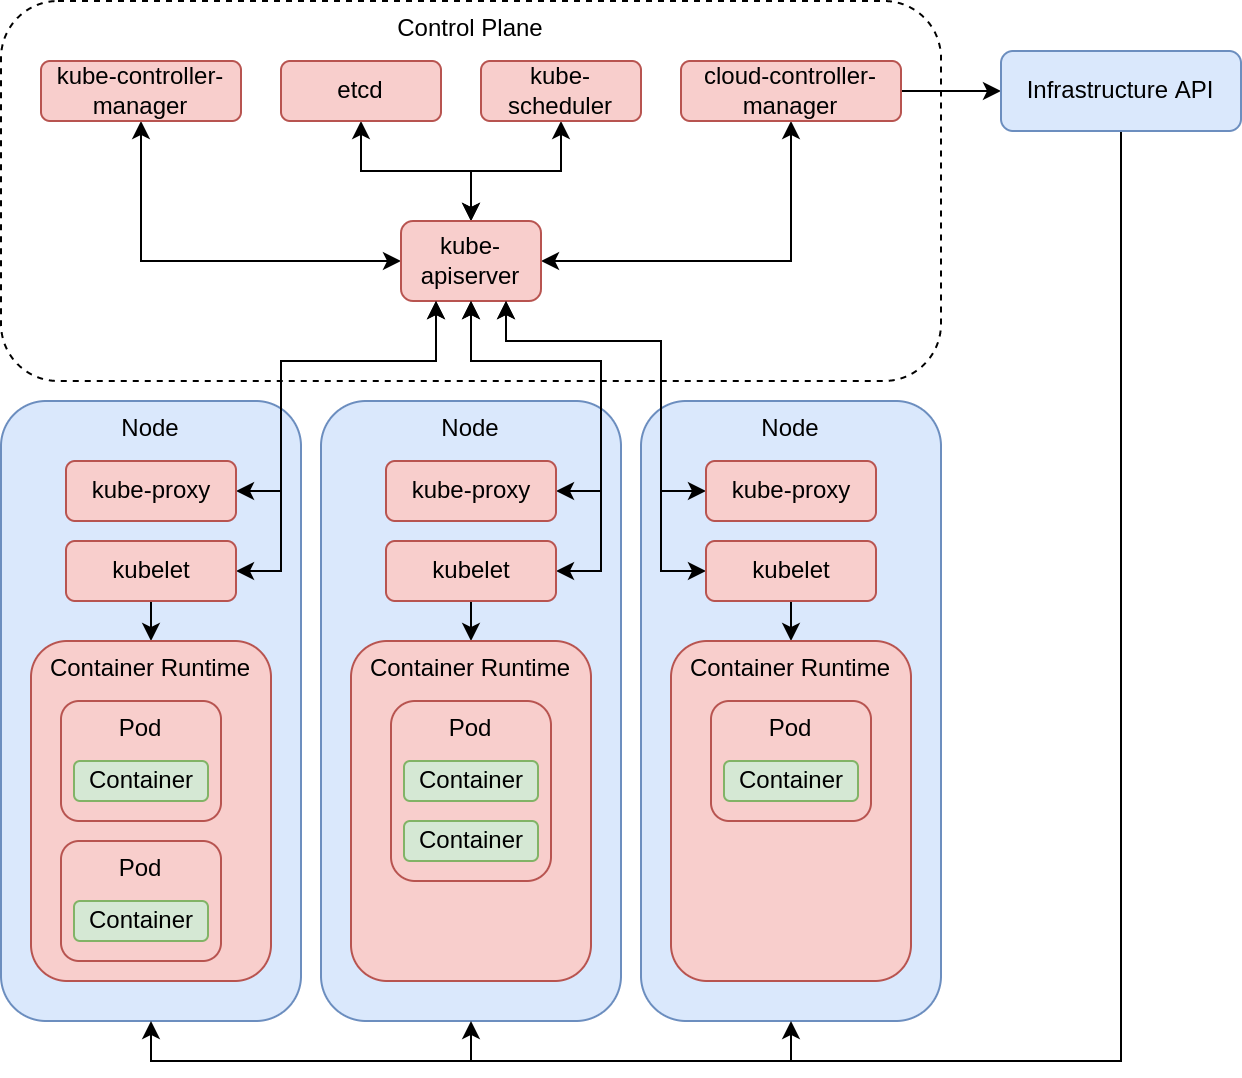
\includegraphics[width=\linewidth]{resources/kubernetes-overview.drawio.png}
  \caption{Overview of core Kubernetes components.}
  \label{fig:kubernetes-overview}
\end{figure}

We will first have look at an overview over the components of a Kubernetes
cluster. Figure \ref{fig:kubernetes-overview} can assist the reader in
understanding the relations between those components.

\begin{description}
  \item[Pods]
    A group of containers that share storage and network resources that models
    an application-specific logical host. The containers that make up a pod are
    always located on the same node and are scheduled in unison.

    In a broader sense, the pods are execution environments in which
    applications, in the form of containers, can be deployed and executed. As
    such, the pods are still part of the Platform layer, execution environments
    managed by an application orchestration service, and the containers
    are the applications of the Application layer.

  \item[Nodes]
    Nodes are machines running containerized applications. On each node run the
    following components: kubelet, container runtime, kube-proxy. The kubelet is
    an agent that is responsible for making sure that all containers of a pod
    are running, while the container runtime is the software that is actually
    responsible for running containers. The kube-proxy component allow the
    discovery of applications running inside the cluster and the exposure of
    those applications as services.

    These nodes correspond to compute resources of the Infrastructure layer. The
    components on those nods however are part of the Platform layer, as they
    implement specific functionalities needed in order to provide the services
    of the Platform layer.

  \item[Control Plane]
    A collection of components that manage nodes and pods inside the cluster,
    making global decisions about the cluster. This includes an API
    (kube-apiserver), a backing store (etcd) for all cluster data, and a
    scheduler (kube-scheduler) that assigns pods to nodes. Kubernetes adopts the
    concept of control loops, enabling the use of so-called controllers, which
    are non-terminating loops that watch the state of the cluster and make
    requests of changes when needed. While each of these controllers are
    logically separate processes, they are compiled into a single
    kube-controller-manager component. The management of Infrastructure layer
    resources is abstracted by the cloud-controller-manager which implements
    cloud specific resource management. All control plane components are also
    deployed in the Kubernetes cluster using pods.

    The components of the control plane implement specific behaviors, which
    together with the components on the nodes, provide the services of the
    Platform layer.
\end{description}

\subsubsection{Infrastructure Management and Security}

Kubernetes enables cloud providers to implement cloud specific infrastructure
management services by developing a cloud-controller-manager, Container Storage
Interface (CSI), and Container Network Interface (CNI), allowing tenants to
automatically scale their Kubernetes cluster depending on the current
utilization of infrastructure resources in order to be more cost-efficient.

The cloud-controller-manager typically consists of multiple components that
create and update load balancers, and manage the lifecycle of nodes.

CSI plugins are responsible for creating, updating, and destroying storage
resources in order to provide pods with persistent storage, referred to as
persistent volumes. Cloud providers often also provide storage encryption
services in conjunction with their storage resources. These encryption services
use keys provided by a KMS. While some cloud providers allow tenants to provide
their own KMS, the encryption service still needs plain text access to keys in
order to encrypt and decrypt data.

CNI plugins create, update, and destroy the underlying network resources of the
Kubernetes cluster and provide node-level, and pod-level communication. Some
CNIs also implement authentication and authorization that allow tenants to
enforce network policies in the cluster, and transparent encryption, protecting
confidential data traversing network resources.

\subsubsection{Application Orchestration}

The basic workflow of how Kubernetes deploys, configures, and starts a pod on a
node is as follows (see Figure \ref{fig:kubernetes-application-orchestration}).
Note that this description of the workflow is greatly simplified.

\begin{figure}[H]
  \centering
  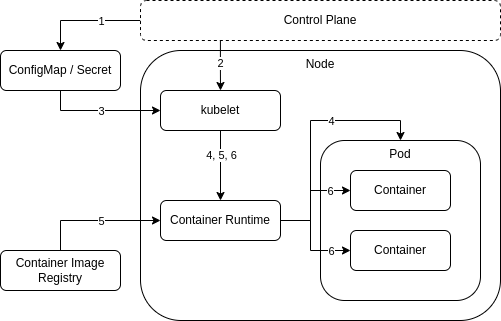
\includegraphics[width=0.7\linewidth]{resources/kubernetes-application-orchestration.drawio.png}
  \caption{Kubernetes' application deployment, configuration, and execution workflow.}
  \label{fig:kubernetes-application-orchestration}
\end{figure}

\begin{enumerate}
  \item Upon request of a tenant, the control plane creates ConfigMaps/Sects,
        which contain non-confidential/confidential configurations of an
        application.
  \item Upon request of a tenant, the control plane requests the kubelet of a
        node to create a pod and provides the kubelet with the specification of
        the pod. This specification includes container images,
        ConfigMaps/Secrets, storage configuration, and network configuration.
  \item Kubelet pulls specified ConfigMaps/Secrets onto the node.
  \item Kubelet calls the container runtime to create the pod, configure its
        storage and network, and provide the pod with the configurations of the
  \item Kubelet calls the container runtime to pull the specified container
        images.
  \item Kubelet calls the container runtime to create and start the application
        containers inside the pod using the pulled container images.
\end{enumerate}

\section{Confidential Computing}
\label{sec:confidential-computing}

Moving on from the traditional distributed computing model, this section gives
an overview of the current state of confidential computing.

Data can be in three distinct states: ``at rest'', ``in transit'', and ``in
use''. These three states describe data stored in persistent storage, traversing
a network, and data currently being processed by an application. While
technologies protecting data at rest and in transit are commonly used today,
there are not many methods to protect data in use.

Confidential computing provides hardware-based primitives that allow the
creation of trusted execution environments (TEEs). These TEEs have specific
properties that protect data in use.

\subsection{Trusted Execution Environments (TEEs)}
\label{sec:tee}

\subsubsection{Properties}

There are different definitions of a trusted execution environment (TEE) with
varying properties. The three main properties defined by the
\textit{Confidential Computing Consortium} \cite{ccc2022technicalanalysis} are:

\begin{description}
  \item[Data confidentiality]
    Prevent unauthorized entities from viewing data that is in use within a TEE.
  \item[Data integrity]
    Prevent unauthorized entities from adding, removing, or changing data while
    it is in use within a TEE.
  \item[Code integrity]
    Prevent unauthorized entities from adding, removing, or changing code
    executed in the TEE.
\end{description}

Besides ensuring the confidentiality of data, code integrity is also critical
for the confidentiality of data. Even if data confidentiality is implemented
correctly, executing compromised code inside TEEs can also lead to confidential
data leakage.

Provided that the application code implements the computation correctly, data
and code integrity ensure that neither the data nor the application has been
modified, allowing clients to trust the results of the computations run inside
TEEs.

As TEE technologies widely differ in their implementations, this thesis will
treat the hardware and software components that create and protect TEEs as a
single platform consisting of all hardware and software components involved, and
refer to it as the ``TEE platform''.

Besides the three core properties, TEE platforms also often provide mechanisms
that enable the integration of a remote attestation process (see Section
\ref{sec:remote-attestation}), enabling clients to assess the trustworthiness of
TEEs created by an untrusted party. These technologies generally produce
evidence about the authenticity and integrity of both the TEE platform and
specific TEEs.

\subsubsection{Hardware Support}

The security of a software layer can only be as strong as the layers below it.
This is why an ideal security solution acts from the lowest layer possible. By
providing security through the lowest layer -- the hardware -- it is possible to
remove almost all software components between the hardware and the TEE from the
list of trusted components, including system software such as the operating
systems and hypervisors. The only components that need to be trusted are the
components of the TEE platform.

Today most TEE implementations still rely on firmware components that are part
of the TEE platform, allows manufacturers to deploy bug fixes and security
patches. Because an untrusted service provider can compromise these firmware
components, TEE platforms generally facilitate hardware-based mechanisms that
produce evidence about the integrity of the TEE platform.

\subsubsection{Memory Protection}

Most TEE technologies today rely on the protection of memory to provide the
three properties defined above. They often implement two mechanisms, protecting
the confidentiality and integrity of data stored in memory:

\begin{description}
  \item[Memory Encryption]
    TEE technologies rely on hardware components to encrypt data that is being
    transferred from the CPU to the physical memory of a machine and decrypt
    data moving from the memory to the CPU. Unlike homomorphic encryption, which
    provides specific computational functions directly on encrypted data
    \cite{monique2013homomorphicencryption}, TEE technologies transparently
    en-/decrypt data. Most importantly, the unencrypted data is only available
    while being processed by the CPU, and is encrypted before leaving the CPU.
    Memory encryption strengthens the confidentiality of data in use, as
    untrusted software components that gain access to the memory of a TEE or
    malicious entities that have physical access to the machine only see
    encrypted data.

  \item[Memory Access Control]
    On the other hand, memory integrity is guaranteed by enforcing that only the
    TEE owning a specific memory region can modify data stored in this region.
    In order to achieve this, the TEE platform has to keep track of protected
    memory pages, and their owners.
\end{description}

\subsection{TEE Models}
\label{sec:tee-models}

There are two distinct models of TEEs, process-based and VM-based.

\subsubsection{Process-based TEEs}
\label{sec:process-based-tees}

Process-based TEEs introduce a new programming model. A program needs to be
split into two components, trusted and untrusted. These are often referred to as
the ``enclave'' and ``host''. The enclave is executed in a TEE and, as such,
should contain all code that interacts with confidential data, whereas the host
component is responsible for handling non-sensitive tasks like networking and
file I/O.

While the host is not shielded, the enclave is protected from the rest of the
system, including:

\begin{itemize}
  \item the enclave's own host
  \item other processes running on the same machine
  \item the operating system
  \item firmware such as the BIOS
  \item the hypervisor and host operating system (in virtualized environments)
  \item hardware other than the processor
\end{itemize}

Splitting a program into enclave and host is challenging. It requires a deep
understanding of security and how these process-based TEE solutions work. SDKs
and frameworks often hide the split between host and enclave from developers to
ease the development of such applications \cite{schuster2022}.

Library OSes like Gramine and Occlum go even further and provide a POSIX-like
runtime environment with network, file I/O, and multithreading support. Because
applications running inside the enclave do not have access to the underlying OS,
library OSes provide libraries that implement OS system calls in the form of
library functions, while a boilerplate host provides I/O functionalities
\cite{tsai2014graphene}.

Even though these SDKs, frameworks, and library OSes ease the development, using
process-based TEEs still requires more development effort, and porting existing
applications often still requires the modification of the application.

\subsubsection{VM-based TEEs}
\label{sec:vm-based-tees}

The central concept of VM-based TEEs is to apply the TEE properties to a whole
virtual machine. Traditionally, hypervisors are fully responsible for managing
VM memory and thus have access to VM memory. On the other hand, TEE platforms
offering VM-based TEEs take away the responsibility of VM memory protection from
the hypervisor because the TEE platform itself already implements memory
protection. So instead of having full access to a VM's memory, the hypervisor
now only manages VM memory through mechanisms offered by the TEE platform.

VM-based TEEs are specifically designed to protect VMs from the rest of the
system, including:

\begin{itemize}
  \item VM firmware (e.g., OVMF)
  \item the hypervisor and/or host operating system
  \item hardware other than the processor
\end{itemize}

\subsubsection{Comparison}

Figure \ref{figure:cc-tee-comparison} compares the list of trusted components of
an application running without confidential computing, inside a process-based
TEE, and inside a VM-based TEE. In both TEE models the TEE platform enforces the
TEE properties and thus the hardware has to be partly trusted. 

On the one hand, process-based TEEs allow fine-grained separation of trust by
splitting applications into host and enclave, but this requires applications to
be ported to a new programming model. On the other hand, VM-based TEEs have much
larger attack surfaces because they include an entire OS but allow complex
applications to be run in a more secure environment without the need to modify
the applications.

\begin{figure}[H]
  \centering
  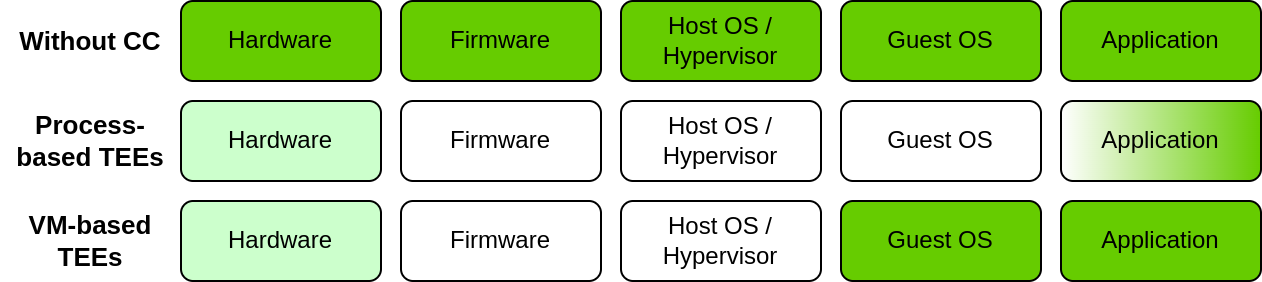
\includegraphics[width=0.85\linewidth]{resources/tee-models-comparison.drawio.png}
  \caption[Comparison of TEE models.]{
    Comparison of TEE models. In both TEE, cases the hardware has to be partly
    trusted, illustrated by the lightly marked hardware components. In the
    process-based TEE model, the application has to be split into enclave and
    host, which is why the application component is marked with a gradient.
  }
  \label{figure:cc-tee-comparison}
\end{figure}

\subsection{Commercially Available TEE Technologies}
\label{sec:commercial-tee-technologies}

\begin{description}
  \item[Intel SGX]
    Intel Software Guard Extensions (SGX) provides process-based TEEs by relying
    on hardware to create enclaves that contain application code and
    confidential data. As the name implies, it is an extension of Intel's CPU
    instruction set architecture \cite{costan2016sgx}.

    The CPU protects a designated memory area called the Processor Reserved
    Memory (PRM) established by SGX by ensuring that other software and hardware
    components, such as system software (hypervisor or OS) and DMA devices, do
    not have access to the PRM. Confidential data and enclave application code
    is stored in the Enclave Page Cache (EPC), a subset of the PRM. SGX relies
    on untrusted system software to manage EPC pages by assigning EPC pages to
    enclaves and evicting these pages if needed. However, system software cannot
    directly access the EPC, and the CPU maintains Enclave Page Cache Map (EPCM)
    in the EPC that keeps track of allocated EPC pages and the enclave which
    owns the page. Using the EPCM, the CPU checks the correctness of the system
    software's allocation decisions, ensures that an EPC page is only assigned
    to a single enclave, and that only the assigned enclave can access and
    modify the EPC page. The CPU also encrypts EPC pages while they are stored
    in physical memory to prevent leaking confidential data through PME attacks
    and guarantee the confidentiality of data stored in EPC pages after
    eviction.

    Initially, the system software asks the CPU to copy data from unprotected
    memory into EPC pages and assigns the pages to the enclave. After the EPC
    pages are loaded, the enclave is marked as initialized, and the system
    software can not access nor modify EPC pages anymore. The CPU then measures
    SGX firmware components and the EPC pages of the enclave, producing
    attestation evidence which is then signed by the CPU using a cryptographic
    key that is only accessible by the CPU. The signature can then be used to
    verify the authenticity of the evidence, which in turn can be used to verify
    the integrity of the enclave and the SGX platform. An attestation can not
    only be requested after initialization but also during runtime.

  \item[AMD SEV]
    AMD SEV-SNP is the latest iteration of AMD's Secure Encrypted Virtualization
    (SEV) technology \cite{amd2021sev, amd2017seves, amd2020sevsnp} and, as the
    name implies, provides VM-based TEEs.

    SEV relies on hardware-embedded encryption engines that encrypt or decrypt
    memory pages written to or read from the physical memory of a machine. It
    utilizes the AMD Secure Processor (AMD-SP), which is integrated into the
    same chip as the CPU, to generate and manage cryptographic keys used for the
    en-/decryption. All software and data are tagged with an Address Space
    Identifier (ASID). The CPU uses the ASID to restrict data access and
    modification to the owner with the same ASID, protecting data from any
    unauthorized usage. However, in the first iteration of SEV, the registers of
    a virtual CPU could be used to leak confidential data when shutting down a
    VM. Subsequently, AMD released their second iteration SEV-ES (Encrypted
    State), which encrypts VM memory and virtual CPU registers. The latest
    version SEV-SNP (Secure Nested Paging), introduced additional features that
    protect VM memory integrity.

    The attestation process for SEV VMs is similar to the attestation process
    for SGX enclaves. A hypervisor launches a VM, and after the VM is fully
    loaded, the VM's memory is encrypted. Subsequently, the AMD-SP measures SEV
    firmware components and VM memory pages, which are signed using a
    cryptographic key only accessible by the CPU. Again, the signature can then
    be used for verifying the authenticity of the measurements, and the
    measurements can be used for verifying the integrity of the VM and the SEV
    platform. Attestation support in SEV and SEV-ES was limited, as measurements
    could only be requested during the launch of a VM. SEV-SNP supports the
    request for measurements at any time, enabling a more flexible remote
    attestation.
\end{description}

\subsection{Limitations}
\label{sec:limitations}

\begin{description}
  \item[Performance Impact]
    Existing solutions require careful configuration to achieve acceptable
    performance or are inappropriate for specific use cases
    \cite{akram2021performance}. For example, due to the limited size of the EPC
    and the restricted programming model, Intel SGX displays a significant
    performance loss for high performance workloads, making the usage of SGX for
    these kinds of cases impractical.
  \item[CPU centric focus]
    Most of today's confidential computing solutions focus on a CPU-level view
    of memory permissions. This limits the application of confidential computing
    to heterogeneous computing systems, where discrete accelerators are used in
    order to speed up specific computations (e.g. GPUs and NPUs for machine
    learning workloads). However, there is ongoing work on integrating
    confidential computing into heterogeneous computing systems
    \cite{jiang2022cronus}.
  \item[New technology that requires further research]
    Since the introduction of Intel SGX in 2015, numerous vulnerabilities have
    been found in the SGX architecture \cite{fei2021sgxvulnerabilities}. AMD SEV
    has also not been spared, which until now required two iterations to fix the
    issues that have been discovered. Both technologies also depend on existing
    software, such as operating systems, hypervisors, and VM firmware, to
    implement the support of these technologies. These implementations also
    require further research and testing to find vulnerabilities and security
    issues.
\end{description}

\section{Remote Attestation}
\label{ch:remote-attestation}

Running applications inside a CC enabled environment is not enough in order to
deepen the trust with the client or third-parties. In order to prove that the
application is running inside a CC enabled environment and that neither the
application nor the system it is running on has been tampered with, the provider
can employ remote attestation.

In a remote attestation environment there are at least two roles: the attester
and the relying party. The attester produces information about itself
(evidence), on which the relying party makes a decision whether to trust the
attester or not.

In our context the attester would be the system running a client application and
the relying party would be the data owner.

\subsection{Remote Attestation Procedures (RATS)}
\label{sec:rats}

\begin{figure}
  \centering
  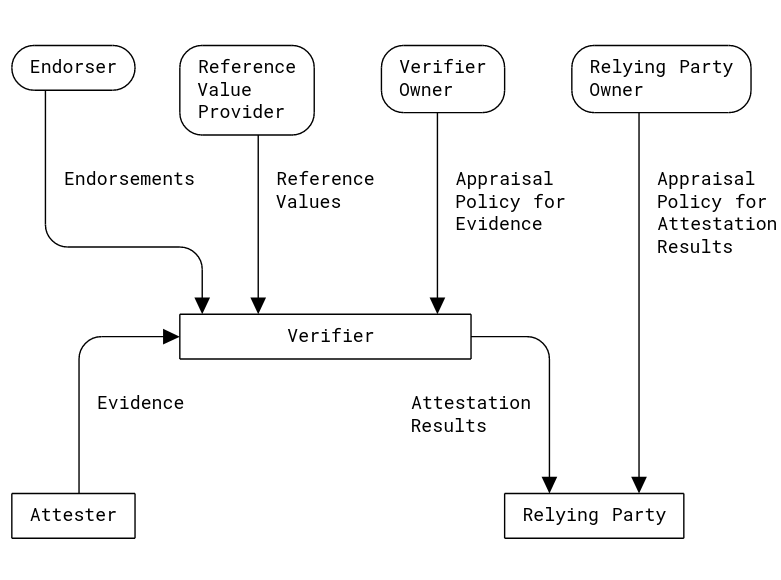
\includegraphics[width=0.7\linewidth]{resources/rats-architecture.png}
  \caption[RATS architectural overview]{
    RATS architectural overview.\\
    Source: \citetitle{rfc9334} \cite{rfc9334}
  }
  \label{figure:rats-architecture}
\end{figure}

Remote Attestation Procedures (RATS) defines a general architecture, roles, and
messages in order to establish trust between the relying party and the attester.
Figure \ref{figure:rats-architecture} shows the general architecture. RATS
introduces few new roles where the most prominent one is the verifier. It
produces attestation results by using evidence, endorsements, reference values,
and applying an appraisal policy to assess the trustworthiness of the attester.
These attestation results then support the decision process of the relying party
on whether to trust the attester or not. We will go into more detail in chapter
\ref{sec:proposal:architecture}.


\chapter{Trusted Distributed Computing Model}
\label{ch:trusted-distributed-computing-model}
Section \ref{sec:traditional-distributed-computing} described the traditional
distributed computing model, where the service provider is trusted by the data
owner, and defined a generalized layered model. This chapter will define a
threat model, identify threats and issues of the Infrastructure and Platform
layers when the service provider becomes untrusted. Subsequently, the new
trusted distributed computing model will be defined, by integrating TEE
technology (see Section \ref{sec:confidential-computing}) and the RATS framework
(see Section \ref{sec:remote-attestation}) into the traditional distributed
computing model. Finally, this chapter demonstrates this new model by looking at
two case studies and evaluates the new model based on the threat model.

\section{Threat Model}
\label{sec:untrusted-threat-model}

\subsection{Infrastructure Layer}

\begin{description}
  \item[Threats from storage resources]
    Storage resources of the Infrastructure layer are typically protected by
    physically securing the location of the hardware and application transparent
    encryption. However, in the trusted distributed computing model the
    service provider is untrusted, and the application owner has to implement
    application level encryption, preventing the service provider gaining plain
    text access to confidential data.

  \item[Threats from networking resources]
    Networking resources offer means of communication. However, in a distributed
    computing environment, these communication channels are often untrusted as
    these resources are shared between multiple tenants. An attacker might gain
    unauthorized access to confidential data shared by an application by
    capturing data from the shared network resources. Applications sharing
    confidential data using untrusted communication channels need to implement
    authentication \cite{lampson1992authentication}, authorization
    \cite{woo1992authorization}, and encryption in order to securely use these
    untrusted communication channels and not leak confidential data to a
    malicious attacker that has access to network resources. Authentication and
    encryption is usually implemented using the Transport Level Security (TLS)
    protocol \cite{rfc5246}, which utilizes a trusted third party (the
    certificate authority) for authentication and the Diffie-Hellman key
    exchange protocol in order to establish a shared secret for encryption.

    Typically, these implementations do not rely on services provided by the
    service provider and as such pose no issues for moving to an untrusted
    distributed computing model.

  \item[Threats from compute resources]
    Techniques for protecting data resting in storage and traversing networking
    resources largely are based on cryptographic primitives, such as encryption,
    one-way hash functions, and digital signatures. All of these primitives
    require some kind of cryptographic key (e.g. secret key for symmetrical
    encryption, private keys for asymmetrical encryption and singing) that need
    to be kept secret. Typically, these keys and the decrypted data are stored
    unprotected in the memory of the machines while in use and is therefore a
    prime target for attacks.

    There are two types of physical attacks, related to the memory of a system,
    summarized by \citeauthor{weis2014protecting} \cite{weis2014protecting}:
    \textsb{Direct Memory Access (DMA) Attacks} exploit the design of the x86
    instruction set architecture that allow hardware subsystems to bypass the
    CPU and directly access the memory of the machine. Like the name implies,
    \textsb{Physical Memory Extraction (PME) Attacks} directly extract data from
    the physical system memory of a machine. Example for this type of attack are
    monitoring the memory bus of a machine, cold boot attacks, and exploiting
    special persistent, nonvolatile memory modules. While software and hardware
    based mitigations to DMA attacks exist, the firmware and software providing
    these mitigations are in control of the service provider. A malicious
    service provider could modify the firmware and software components to only
    pretend to mitigate those threats. In the past there were no countermeasures
    for PME attacks available (today confidential computing tries to address
    this issue \ref{sec:confidential-computing}).

    One primary benefit that virtualization brings is isolation with the goal of
    shielding a VM from other VMs. Traditionally, the hypervisor is assumed to
    be trusted. As such it has been a high-privileged software component
    responsible for the virtualization of a VM's CPU, mapping of a VM's
    virtualized physical memory address space to the host machines physical
    memory address space, and intercepting and carrying out privileged
    operations invoked by a VM, in order to provide VM management tasks such as
    starting, stopping, suspending, restoring, and migrating VMs. But a
    malicious administrator or an attacker that gained access to hypervisor
    level privileges by exploiting vulnerabilities can completely monitor and
    modify resources available to another VM that may contain confidential data.
    Over the years there have been many vulnerabilities found in commonly used
    hypervisors that break the isolation promises of hypervisors
    \cite{perezbotero2013hypervisorvulnerabilities,
      reuben2007surveyvirtualmachinesecurity}. We will refer to this kind of
    attacks as \textsb{Virtualization-based Attacks}.

    Measures for protecting VM's from the hypervisor mostly separate the high
    privileged operations into a small component, that is either implemented in
    hardware or as a software component, that control the access to these
    operations and move the rest of the hypervisor into a less privileged
    execution mode \cite{jin2011securevirtualization,
    szefer2012hypvervisorsecurevirtualization, li2019protectingvmfromhypervisor,
    mi2020disaggregatednestedvirtualization}. However, all of these mitigations
    are based on the trust that the party managing the hypervisor properly
    selects, configures, and patches the hypervisor. There are often no means
    for application owners to enforce or verify the selection, configuration,
    and update policies or and are also not able confirm that the hypervisor has
    not been tampered with.

    Aside from physical threats, \citeauthor{weis2014protecting} also describes
    the threat of \textsb{Boot Integrity (BI) Attacks}. While the operating
    system of a machine can often be provided by the application owner,
    firmware, such as the BIOS, used in both physical and virtual environments
    providing hardware abstraction, are often controlled by the service
    provider. Consequently, BI attacks are applicable in physical and virtual
    environments. BI attacks exploit the high level of privilege and the fact,
    that firmware may be invisible to the operating system, in order to
    compromise security measures in higher levels of software. As such,
    establishing trust in the provided machines requires every piece of software
    that is executed during the lifetime (including the firmware) of the
    machines to be measured, verified, or isolated.

    There have been two main approaches to prevent BI attacks:

    The \textsb{Secure Boot} approach verifies the signatures of each software
    component loaded during the boot process of a machine. This requires the
    maintenance of a certificate which is used to verify the signatures of the
    firmware, bootloader, and kernel of the operating system.

    But Secure Boot does not provide means to know what specific components
    loaded during the boot process, only that those components are verified
    using the provided certificate. \textsb{Measured Boot} aims to provide a
    trusted record of the boot process. Traditionally, this has been done using
    a Trusted Platform Module (TPM) which contains Platform Configuration
    Registries (PCRs) that are used to store measurements of loaded software
    components. These measurements are taken by various software components,
    such as the firmware, or bootloader. After the boot the PCRs are sealed,
    preventing the modification of the measurements, and signed by the TPM.
    Measured Boot then relies on a remote attestation process (see Section
    \ref{sec:remote-attestation}), to recover the signed set of measurements,
    verify the signature, and evaluate whether the measurements follow a known
    policy.

    Secure boot and Measured Boot rely on a trusted software component to verify
    and/or measure other software components required for the boot process.
    However, in an untrusted infrastructure environment tenants can not trust
    these components, as these can be modified by the service provider.
\end{description}

\begin{table}[H]
  \centering
  \scriptsize
  \begin{tabularx}{\linewidth}{
    | p{8em}
    | >{\raggedright\arraybackslash}X
    | >{\raggedright\arraybackslash}X
    | >{\raggedright\arraybackslash}X
    |
  }
  \hline
  Resource          & Threat                                      & Mitigation                                                                                              & Issue                                                                                                                               \\
  \hline
  \hline
  Storage Resources & Access of data resting in storage resources & Application level encryption of data resting in storage resources                                       &                                                                                                                                     \\
  \hline
  Network Resources & Access of data traversing network resources & Application level authentication and authorization, and encryption of data traversing network resources &                                                                                                                                     \\
  \hline
  Compute Resources & DMA attacks                                 & Software and Hardware based mitigations available                                                       & Lack of a trusted component that can verify that mitigation is working as intended                                                  \\
  \cline{2-4}
                    & PME attacks                                 &                                                                                                         & No mitigation                                                                                                                       \\
  \cline{2-4}
                    & Virtualization-based attacks                & Properly selected, configured, patched, and unmodified hypervisor                                       & Lack of trusted component that can enforce or verify the selection, configuration, update policies, and integrity of the hypervisor \\
  \cline{2-4}
                    & BI attacks                                  & Secure Boot \& \newline Measured Boot                                                                   & Lack of a trusted component that can perform measurements and/or verification                                                       \\
  \hline
\end{tabularx}

  \caption{Overview of Infrastructure layer threats, typical mitigations in the traditional distributed computing model, and arising issues when moving to the trusted distributed computing model.}
  \label{table:threats-overview}
\end{table}

\subsection{Platform Layer}

\begin{description}[style=standard]
  \item[Infrastructure management services] typically have full access to
    Infrastructure layer resources. Therefore, the same threats of the
    Infrastructure layer apply here.

  \item[Security services] offer application-level authentication,
    authorization, and/or encryption, support the process of implementing
    security into an application. However, a malicious service provider might
    modify or access those services in order to use another user's credentials
    (Spoofing), gain privileged access to resources and services (Elevation of
    Privilege), and/or gain plain text access to confidential data.

  \item[Monitoring and Logging services] aggregating metrics and logs of
    applications in the Platform layer. While monitoring metrics usually do not
    contain sensitive information, the application logs can in some cases
    contain sensitive information.

  \item[Application orchestration services] automate the process of preparing
    target execution environments, and installing, configuring, and maintaining
    applications inside the target environments.
    
    A malicious service provider might misuse application orchestration services
    in order to:

    \begin{itemize}
      \item execute malicious code in the provided target environments.
      \item modify applications or their configurations, directly influencing
            the behavior of those applications.
    \end{itemize}
\end{description}

\begin{table}[H]
  \centering
  \scriptsize
  \begin{tabularx}{0.7\linewidth}{
    | p{15em}
    | >{\raggedright\arraybackslash}X
    |
  }
  \hline
  Service Type                       & Issue                                                       \\
  \hline
  \hline
  Infrastructure Management Services & Same as Infrastructure layer                                \\
  \hline
  Security Services                  & Spoofing, Elevation of Privilege, plain text access         \\
  \hline
  Monitoring \& Logging Services     & Access to possibly sensitive logs                           \\
  \hline
  Application Orchestration Services & Execution of malicious code in target execution environment \\
  \cline{2-2}
                                     & Modification of applications or their configurations        \\
  \hline
\end{tabularx}

  \caption{Issues in the Platform layer when moving to an trusted distributed computing model.}
\end{table}

\section{Trust Model}

The roles of the trusted distributed computing model are still present, with the
difference that the service provider is no longer consider trusted. However,
there are now three new roles present, based on the RATS framework, and the
service provider is given additional responsibilities:

\begin{description}
  \item[Hardware Manufacturer]
    The hardware manufacturer provides hardware to the service provider that
    form the base for the Infrastructure layer. The hardware has to be able to
    provide TEEs and the hardware manufacturer endorses the security of those
    TEEs. As such the hardware manufacturer takes on the endorser role defined
    by RATS (see Section \ref{sec:remote-attestation}). Even though, this model
    still applies when multiple TEE platforms and hardware manufacturers are
    present, for simplicity we will assume that only a single TEE platform and
    hardware manufacturer is present.

  \item[Service Provider]
    In this model service providers not only provides Infrastructure layer
    resources and manages Platform layer services, but now utilize a TEE
    platform provided by the hardware manufacturer in order to offer the
    capability of creating TEEs and getting evidence for the integrity of the
    TEEs. These TEEs will be used by the application owner to execute
    applications in a trusted environment.

  \item[Reference Value Provider]
    Reference value providers generate reference value of TEEs in advance,
    which is then used by the verifier in order to validate TEEs offered by the
    service provider.

  \item[Verifier Owner]
    An entity that operates the verifier, a new component introduced in this
    model that is responsible for assessing the trustworthiness of TEEs provided
    by service providers.

  \item[Application Owner]
    The responsibilities of application owners did not change. However, because
    in this model the service provider is untrusted, services of the Platform
    layer are also untrusted. As such, the application owner has to ensure that
    the security of the Application layer does not depend on services of the
    Platform layer.
\end{description}

In this model, the service provider is the only role that is not trusted by the
data owner. Because every other role is trusted, a single entity or organization
can take on multiple roles. However, the entity taking on the role of the
service provider can not take on any other roles.

\section{Architectural Overview}

\subsection{Verifier}

The verifier is a required component of the trusted distributed computing
model, responsible for verifying TEE integrity and is operated by the verifier.
When a relying party, usually the application or data owner, requests the
verification of an TEE, the verifier validates that the of evidence provided by
the service provider is produced by the TEE platform using endorsements from the
hardware manufacturer, and verifies the integrity of the TEE using the evidence
and reference values provided by the reference value provider.

Software components involved in the creation process of TEEs, such as firmware
components of the TEE platform or VM firmware, are still under control of the
service provider. So in order for the verifier to validate the integrity of the
TEE, evidence produced by the TEE platform also has to include measurements of
said software components that have to be compared to reference values in order
to verify the integrity of those components.

The verifier is only responsible for verifying the integrity of TEEs as a whole
and does not verify single applications inside TEEs. The verification of
applications inside TEEs is only a side effect of verifying TEEs as a whole.

\subsection{Infrastructure Layer}

\begin{figure}[H]
  \centering
  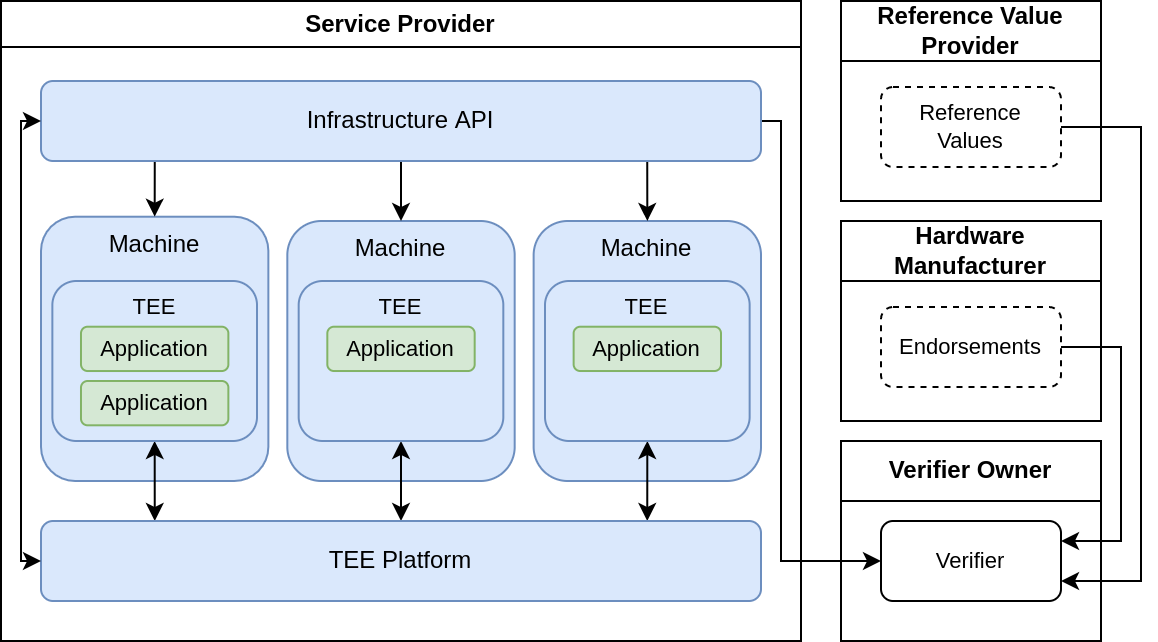
\includegraphics[width=0.9\linewidth]{resources/untrusted-infrastructure-architecture.drawio.png}
  \caption{Overview of the infrastructure in the trusted distributed computing model.}
  \label{fig:untrusted-architecture-overview}
\end{figure}

As outlined in the threat model, protection of data resting in storage resources
and traversing network resources has to be implemented at application level
using authentication, authorization, and encryption.

Instead of directly running applications on provided (physical or virtual)
machines, the data and application owner rely on TEEs to protect data that is
currently in use by applications. In Section \ref{sec:confidential-computing} we
have seen two TEE models. On one hand, a service provider can provide machines
capable of creating process-based TEEs inside those machines, on the other hand,
a service provider can also provide VM-based TEEs, in which case the machine
itself is the TEE.

The TEE platform has to be capable to produce evidence of software components
that have direct access and/or control the access to the memory of a TEE, such
as VM firmware and firmware components of the TEE platform. While the TEE
platform is operated by the service provider, the TEE platform is provided to
the service provided and endorsed by the hardware manufacturer.

A secure channel is essential for data owners to supply applications inside TEEs
with confidential data. Section \ref{sec:ra-secure-communication-channel}
outlined the basic process of establishing a secure communication channel
between the attester and the relying party during the remote attestation
process.

\subsection{Platform Layer}

Like in the traditional distributed computing model, the Platform layer builds
on top of the Infrastructure layer. Therefore, this section assumes the presence
of a TEE platform that can be used to securely deploy applications and provide
the application with confidential data.

Because in this model the service provider is untrusted, there are three
possible solutions to the issues of the services typically located in the
Platform layer:

\begin{itemize}
  \item Moving these services to the Application layer or directly implementing
        the tasks that these services take on into applications.
  \item Management of the service by a trusted party that is not the application
        owner (otherwise it would mean that the service is in the application
        layer).
  \item Splitting the service into a privileged and unprivileged part. The
        unprivileged part can still be operated by the service provider, while
        the privileged part has to be managed by the application owner.
\end{itemize}

The first option can be applied to all services of the Platform layer, as such
this section will focus on the evaluation of each previously defined service
type based on the latter two options.

\begin{description}[style=standard]
  \item[Infrastructure Management Services] do not need to be modified and can
    still be managed by the service provider, assuming applications are
    adequately shielded from Infrastructure layer resources as described in the
    previous section.

  \item[Security Services] can not be managed by an untrusted party, as
    application-level security depends on those services. Management of
    identities, administration of authentication policies, and encryption and
    decryption of data are all privileged tasks. Therefore, splitting security
    services into unprivileged and privileged parts is not feasible and these
    services have to managed by a trusted party.

  \item[Monitoring and Logging Services] can be managed by a service provider,
    assuming that application logs do not include sensitive information or are
    protected (e.g. encrypting or obfuscating logs).

  \item[Application Orchestration Services] are a more complex topic. Because
    the TEE platform is still under control of the service provider, software
    responsible for managing TEEs are still untrusted (e.g. hypervisor, OS
    managing process-based TEEs). Applications and application configurations
    can also be modified by an attacker during the deployment of applications
    into TEEs. Therefore, TEEs, applications, and application configurations
    have to be verified before supplying applications with confidential data.

    There are two ways on how applications can be deployed into TEEs:

    The first option is to create an application package that can be directly
    deployed by the TEE platform. For example the application owner might
    package an application including its (non-confidential) configuration
    directly into an VM image that can be deployed by the service provider. The
    application owner has to provide reference values in the form of
    measurements of the VM, in order for the verifier to verify the integrity of
    the VM including the applications inside. This option moves the installation
    and configuration of applications into the application packaging process,
    and therefore requires a more complex packaging solution. However, it also
    allows the combined verification of TEEs, applications, and application
    configurations.

    The second option is to first create a generic application-agnostic TEE and
    subsequently deploy the application including its (non-confidential)
    configuration into the TEE after verifying its integrity. For example a
    service provider might provide a curated list of generic VM images that can
    be deployed by tenants as VM-based TEEs. A reference value provider has to
    deploy such a VM image, check its content for malicious software, and create
    measurements of the VM beforehand, producing reference values. After a
    VM-based TEE is created, the verifier has to verify the integrity of the
    VM-based TEE using the reference values, after which the application owner
    installs, configures, and executes applications in the verified VM. This
    option decouples the creation of TEEs from the installation, configuration,
    and execution of applications, allowing another reference value provider to
    maintain reference values for TEEs. However, this also decouples the
    verification of TEEs from the verification of applications and their
    configurations, requiring two separate verifications.

    While in both cases the service provider creates TEEs, the service provider
    is not involved in the installation, configuration, and execution of
    applications in the provided TEEs. Both options also require a secure way to
    supply the applications with confidential data, which can again be achieved
    by establishing a secure communication channel during the remote attestation
    process.
\end{description}

\subsection{Application Layer}

The threat model above already discussed how application level authentication,
authorization, and encryption of confidential data is crucial to protect data
resting in storage resources and traversing network resources. As the service
provider is not trusted, Infrastructure and Platform layer protection methods
can not be used, and the application owner has to implement these protections
into the Application layer.

\section{Requirements}
\label{sec:requirements}

This section summarizes the changes made to the traditional distributed
computing model and defines requirements for the trusted distributed computing
model.

The trusted distributed computing model is largely based on concepts of the
confidential computing model and requires a hardware manufacturer to provide:

\begin{enumerate}[label*=R\arabic*]
  \item a TEE platform, capable of creating TEEs and generating evidence, based
        on hardware mechanisms.
  \item endorsements that vouch for the TEE platform's capability to securely
        generate evidence and protect the confidentiality and integrity of TEEs.
\end{enumerate}

There are two requirements for the offerings of a service provider. The service
provider has to provide:

\begin{enumerate}[resume,label*=R\arabic*]
  \item the ability to create TEEs using the TEE platform provided by the hardware
        manufacturer.
  \item the raw evidence produced and signed by the TEE platform that includes:
        \begin{enumerate}[label*=.\arabic*]
          \item measurements of the content of the TEE.
          \item measurements of software components that have direct access or
                the access to the memory TEEs.
        \end{enumerate}
\end{enumerate}

The latter requirement enables the verifier to verify TEEs, preventing the
service provider to tamper with provided TEEs in order to break the
confidentiality and integrity guarantees. This leads to the requirements for the
verifier. The verifier has to verify

\begin{enumerate}[resume,label*=R\arabic*]
  \item the integrity of provided TEEs using measurements provided by the
        service provider and reference values from the reference value provider.
  \item the integrity of the TEE platform by verifying:
        \begin{enumerate}[label*=.\arabic*]
          \item the authenticity of the evidence using the evidence's signature
                and endorsements from the hardware manufacturer.
          \item the integrity of software components that have direct access or
                control the access to the memory of TEEs using measurements of
                those components and reference values from a reference value
                provider.
        \end{enumerate}
\end{enumerate}

While TEEs protect data currently in use by applications, data resting in
storage resources and traversing network resources also have to protected. The
application management process also has to be secured, preventing the service
provider to execute malicious applications inside TEEs and modifying
applications before they are deployed into TEEs. This results in the following
requirements for the application owner. The application owner has to:

\begin{enumerate}[resume,label*=R\arabic*]
  \item implement security (authentication, authorization, and encryption) in
        the Application layer, not relying on security services provided by the
        Platform layer.
  \item protect application logs by removing, encrypting, or obfuscating
        confidential information from the logs.
  \item deploy applications inside TEEs. This includes:
        \begin{enumerate}[label*=.\arabic*]
          \item providing reference values for applications and their
                configuration.
          \item installing, configuring, and executing applications inside TEEs.
          \item securely supplying applications with confidential data only
                after verification of applications and their surrounding TEE
                (e.g. by establishing a secure communication channel during the
                remote attestation process).
        \end{enumerate}
\end{enumerate}

%%%%%%%%%%%%%%%%%%%%%%%%%%%%%%%%%%%%%%%%%%%%%%%%%%%%%%%%%%%%%%%%%%%%%%%%%%%%%%%%
% Evaluation
%%%%%%%%%%%%%%%%%%%%%%%%%%%%%%%%%%%%%%%%%%%%%%%%%%%%%%%%%%%%%%%%%%%%%%%%%%%%%%%%

\section{Evaluation}
\label{sec:evaluation}

This section evaluates the requirements of the trusted distributed computing
model based on the threat model defined in section
\ref{sec:untrusted-threat-model}.

Infrastructure layer threats from storage and network resources are addressed in
the trusted distributed computing model by R7. By implementing authentication,
authorization, and encryption at application level, an attacker that gained
access to storage and network resources or the untrusted service provider
providing these resources, still do not have plain text access to confidential
data.

Threats from compute resources of the Infrastructure layer are addressed by
R1-R6. The issue of traditional mitigations of these threats was the lack of a
trusted component that can verify the integrity of components that implement the
mitigations. R3 and R4 require the service provider to offer the capability to
create TEEs using and get evidence produced and signed by a TEE platform. The
TEE platform is provided and endorsed by the hardware manufacturer (R1 and R2).
Section \ref{sec:confidential-computing} described how TEEs protect memory
confidentiality and integrity using memory encryption and access control.

Physical access to a machine's memory (DMA and PME attacks) are prevented as
data leaving the CPU is encrypted before storing it in memory. As such, an
attacker with direct access to a machine's memory still does not have plain text
access to the data.

Virtualization-based attacks are also mitigated by the TEE platform. VM-based
TEEs split of the memory access control and isolation part of the hypervisor of
into the TEE platform. The hypervisor is still provided with interfaces in order
to manage VMs (e.g. starting, stopping, suspending), but the isolation guarantee
is provided by the TEE platform. And while the hypervisor is also tasked with
managing VM memory (e.g. attaching and releasing), the hypervisor can not read
the memory as it is encrypted.

Measurements produced by the TEE platform can also be used for the measured boot
process mitigating BI attacks against VM-based TEEs. Ongoing work in QEMU, an
open source emulator that can facilitate hardware-assisted virtualization in
order to run VMs, the open virtual machine firmware (OVMF), and the Linux kernel
enable the verification of all components involved in the boot process of an AMD
SEV based VM (see Section \ref{sec:commercial-tee-technologies}). The basic boot
process works as follows: When a VM is started, the AMD-SP measures the VM's
firmware (OVMF), which in turn measures and verifies the integrity of the Linux
kernel. After the VM has booted, the Linux kernel is supplied with an
attestation report that contains a measurement of OVMF, which are relayed to the
verifier in order to verify OVMF's integrity. The attestation report also
contains evidence about the integrity of SEV's firmware components which
together with the measured boot process fulfill requirements R4, allowing a
verifier that supports the verification of SEV's attestation report to fulfill
R5 and R6.

The TEE creation capability of process-based TEE platforms can often be passed
through to VMs (e.g. in the case of Intel SGX), in which case the VM itself and
the hypervisor are not considered trusted. Again, isolation is provided by the
TEE platform (R3), and not the hypervisor. In this model, compromising the VM on
which the process-based TEE is deployed only threatens the availability of the
application, and not the confidentiality of the application's data. TEE
platforms based on the process-based TEE model, still need to provide
measurements of software components of the TEE platform and the TEEs (R4),
allowing a verifier to verify the integrity of the TEE platform (R6) and TEEs
(R5).

R7 requires the implementation of security mechanisms in the Application layer.
These mechanisms can not be based on security services provided by the Platform
layer, as this would allow spoofing and elevation of privilege attacks, or plain
text access to confidential data from the untrusted service provider. While R8
does not require moving monitoring and logging services into the application
layer, it does require the Application layer to protect sensitive information in
application logs. Infrastructure management services can still be part of the
Platform layer, as confidential is already protected from Infrastructure layer
resources by R1-R7.

Application orchestration however, still relies on management of target
environments for applications to be managed by untrusted software components.
That is VM-based TEEs managed by a hypervisor or process-based TEEs managed by
the surrounding host (or guest) OS. R9 requires that the rest of the application
orchestration process, that is installation, configuration, and execution of
applications inside provided target environments, is managed by the application
owner. It also requires the verification of both TEEs and applications before
supplying applications with confidential data. Requiring the verification of
applications enables the detection of modification of applications or their
configurations, and requiring the application owner to manage the execution of
applications inside verified TEEs, prevents the service provider to execute
malicious code.

On the one hand, all R7-R9 remove the service provider as a trusted party, but
on the other hand they significantly increase the responsibilities of
application owners and the size of the Application layer.

%%%%%%%%%%%%%%%%%%%%%%%%%%%%%%%%%%%%%%%%%%%%%%%%%%%%%%%%%%%%%%%%%%%%%%%%%%%%%%%%
% Case Studies
%%%%%%%%%%%%%%%%%%%%%%%%%%%%%%%%%%%%%%%%%%%%%%%%%%%%%%%%%%%%%%%%%%%%%%%%%%%%%%%%

\section{Case Studies}
\label{sec:case-studies}

\subsection{Case Study: Constellation}

Constellation is a project maintained by Edgeless
Systems\footnote{\url{https://docs.edgeless.systems/constellation/}}. By
extending Kubernetes, Constellation provides a platform base that includes
infrastructure management and application orchestration services (see Section
\ref{sec:example-kubernetes}) on top of the Infrastructure layer provided by an
untrusted cloud provider. Its contribution is the protection of the whole
Kubernetes cluster from underlying Infrastructure layer resources by utilizing
VM-based TEEs, and providing transparent network and storage encryption.

\begin{figure}[H]
  \centering
  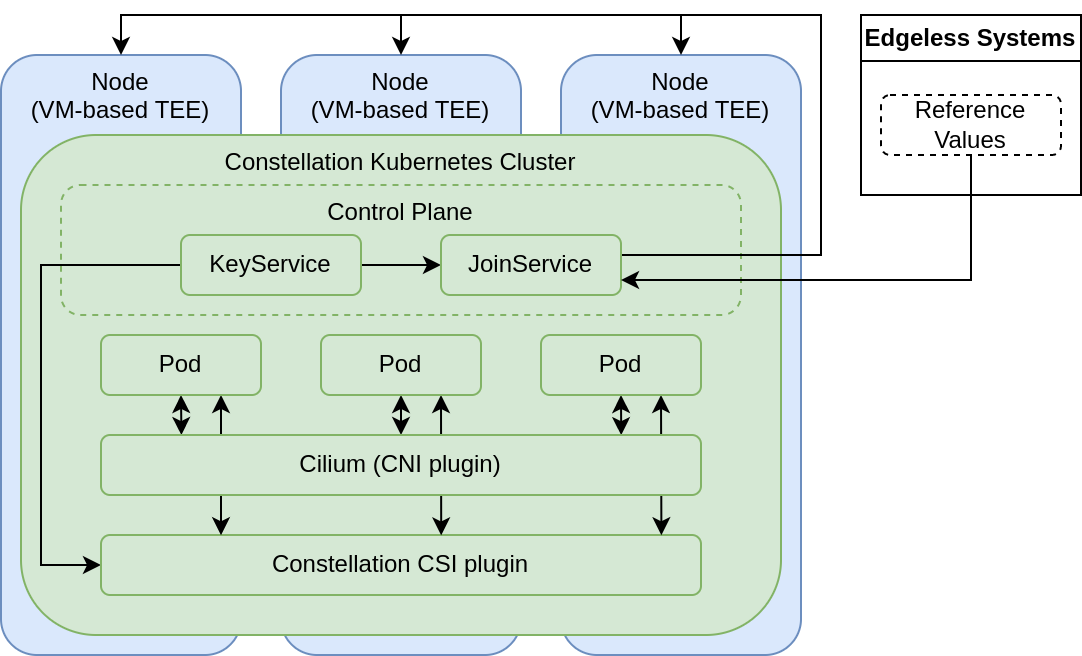
\includegraphics[width=0.8\linewidth]{resources/constellation-kubernetes.drawio.png}
  \caption{Constellation Kubernetes overview.}
\end{figure}

In order to protect data currently in use by control plane components and
application pods, Constellation runs the whole cluster on VM-based TEEs. The
JoinService, a new component of the control plane, is responsible for verifying
new nodes joining the cluster. After a node that is supposed to run control
plane components is verified and joins the cluster, it is supplied by the
JoinService with encryption keys supplied by the KeyService. These keys are then
used to encrypt etcd data that is stored on the node, protecting control plane
data at rest.

In this architecture, the JoinService correlates to the verifier introduced
previously. It uses reference values provided by Edgeless Systems in order to
verify joining nodes. The KeyService manages cryptographic keys used for
encryption and decryption and is therefore a security service.

Protection of control plane and application data in transit is provided by
cilium, the CNI plugin chosen by constellation, which encrypts data exchanged
between pods without the need for applications running inside pods to be
modified. Persistent application data at rest is shielded by the CSI plugin
provided by Constellation, which encrypts and decrypts persistent volumes using
keys provided by the KeyService without needing modification of the applications
inside pods. Both the CNI and the CSI plugin are implementations of
infrastructure and security services

Constellation currently only supports AMD SEV, making AMD take on the role of
hardware manufacturer that provides and endorses the TEE platform (R1 and R2).
However, the currently supported cloud providers (Azure, GCP, AWS) do not fully
support the trusted distributed computing model at the time of writing. For
example AWS currently does not provide the capability of providing SEV based
VMs, not meeting R3. While Azure and GCP provide SEV based VMs, Azure currently
does not provide reviewable VM firmware, not meeting R4.2, and GCP does not
provide evidence produced by the SEV platform, not meeting R4.

Because the cloud providers do not meet R3 and R4, the verifier in the
Constellation architecture (JoinService) can not fulfill R5 and R6. On the one
hand, if the cloud provider does not meet R3, there are no TEEs to be verified,
making complying with R5 impossible. On the other hand, if the cloud provider
does not meet R4, the verifier can not fully verify the integrity of the TEE
platform or TEE, preventing the verifier to satisfy R6.

While Edgeless Systems provides application owners with tools to create and
manage a Constellation Kubernetes cluster, the cluster still has to be
administered by the application owner, putting the whole cluster into the
Application layer. In doing so Constellation meets requirements R7 and R9,
because security services (KeyService, CNI, and CSI plugin) and application
orchestration services (natively included in Kubernetes) are now managed by the
application owner.

\subsection{Case Study: Confidential Containers}

Confidential Containers is another project, trying to implement the untrusted
distributed computing model into the Kubernetes
architecture\footnote{\url{https://github.com/confidential-containers/documentation}}.
The key difference, is that while Constellation applies confidentiality at the
node level, Confidential Containers applies confidentiality at a pod level. By
running containers inside TEEs (both VM-based and process-based) and not the
whole cluster, Confidential Containers goal is to separate the trust model of
the Kubernetes cluster from the applications deployed in the cluster. The
project is still in a very early development stage, as such information provided
in this section is subject to change.

The current Kubernetes architecture puts the container runtime in charge of
managing pods and containers inside the pod (see Section
\ref{sec:example-kubernetes}). Confidential Containers introduces a new
component into the pod: the enclave agent. The enclave agent collects claims
generated by the TEE platform, performs the remote attestation process, receives
confidential configuration and data, pulls container images from the container
image registry, and manages the lifecycle of containers inside the pod. In the
case of VM-based TEEs, a pod is represented by a single VM, which includes the
enclave agent as a process that is started at boot and the containers are
started inside the VM. For process-based TEEs, the enclave agent is a separate
process-based TEE, that creates distinct process-based TEEs for each container
on the node itself. In this case study we will illustrate the Confidential
Container architecture only using VM-based TEEs.

\begin{figure}[H]
  \centering
  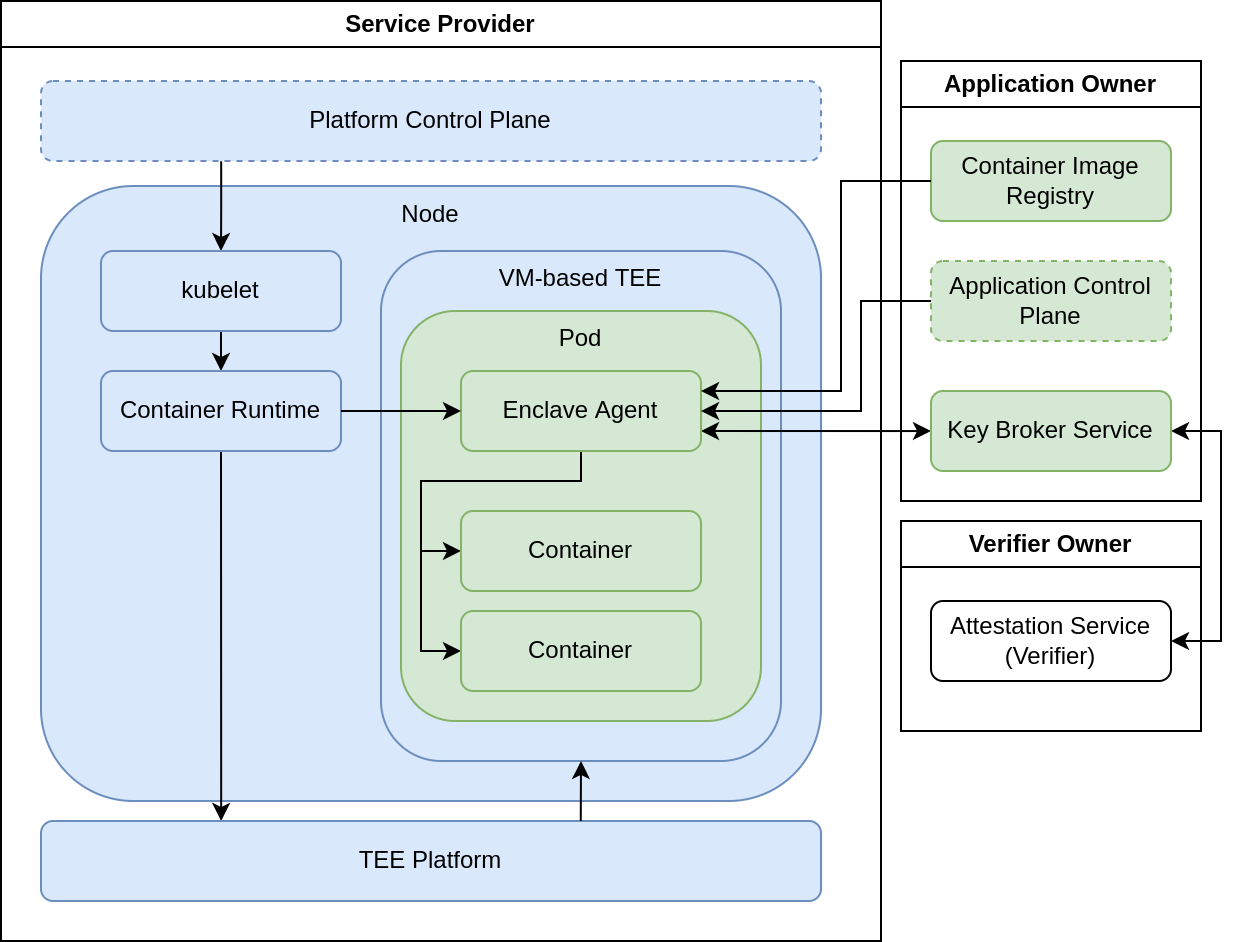
\includegraphics[width=0.8\linewidth]{resources/confidential-containers.drawio.png}
  \caption{Confidential Containers application orchestration overview.}
\end{figure}

While the agent only acts upon request from a single API source, traditionally
the Kubernetes control plane, Confidential Containers is currently working on
splitting the Kubernetes control plane into a trusted and an untrusted part. The
platform control plane (untrusted) would be responsible for unprivileged tasks,
such as infrastructure and TEE management. On the other hand, the application
control plane (trusted) performs privileged tasks, including container
management inside TEEs provided by the platform control plane. The split of the
control plane is enforced by the enclave agent, by blocking privileged actions
originating from the platform control plane, such as creating a malicious
container in a pod, and establishing a secure communication channel to the
application control plane.

The architecture builds upon the assumption that confidential data is provided
to the pod using persistent volumes managed by a CSI plugin, but stored in an
encrypted form. Decryption keys are provided to pods by the key broker service,
which correlates to the relying party of the RATS framework. It receives
evidence from the enclave agent, relays the evidence to the verifier (called
attestation service in the Confidential Containers architecture) for
verification, applies appraisal policies on the returned attestation results,
and releases keys to the enclave agent. During the remote attestation process, a
secure communication channel between the key broker service and the enclave
agent is established, which is used for the secure release of keys to the
enclave agent. Besides data decryption keys the key broker service also sends
communication keys to the enclave agent that are used to establish a secure
communication to other components, such as the application control plane.

Currently, it is still not clear, how the ConfigMap and Secret resources of the
traditional Kubernetes architecture fit into this new architecture, which is why
the following illustration of the application orchestration process does not
include ConfigMaps and Secrets.

\begin{enumerate}
  \item Upon request of a tenant, the platform control plane requests the
        kubelet of a node to create a pod and provides the kubelet with the
        specification of the pod. This specification mainly includes container
        images, storage configuration, and network configuration.
  \item Kubelet calls the container runtime to create the pod and configure its
        storage and network.
  \item The container runtime in turn calls the TEE platform to create a
        VM-based TEE using a predefined VM image that includes the enclave
        agent.
  \item During the boot of the VM the TEE platform produces signed evidence that
        is then passed to the enclave agent after the VM has fully booted. The
        container runtime also passes the pod specifications to the enclave
        agent.
  \item The enclave agent requests the release of keys from the key broker
        service and includes the evidence in the request.
  \item The key broker service relays the evidence to the attestation service
        and receives an attestation result, upon which the key broker service
        applies its own appraisal policy.
  \item If the attestation was successful, the key broker service releases keys
        and a pod specification policy to the enclave agent. The policy can for
        example include storage and network configuration, a container image
        whitelist, a certificate which can be used to validate the authenticity
        of container images.
  \item The enclave agent then compares the pod specification it received from
        the container runtime to the policy. If the specification passes the
        policy, the enclave agent pulls the specified container images and
        validates the signature using the certificate included in the policy.
  \item Only after passing the policy the enclave agent creates the containers
        inside the VM and provides them with decryption keys.
\end{enumerate}

Note that the enclave agent is only trusted, because it is included in the VM
image which is verified by the verifier. Modification of the enclave agent (or
any other software in the VM image) would fail the verification and lead to the
key broker service not releasing keys to the enclave agent.


\chapter{Conclusion}
%% LaTeX2e class for student theses
%% sections/conclusion.tex
%% 
%% Karlsruhe Institute of Technology
%% Institute for Program Structures and Data Organization
%% Chair for Software Design and Quality (SDQ)
%%
%% Dr.-Ing. Erik Burger
%% burger@kit.edu
%%
%% Version 1.3.6, 2022-09-28

\chapter{Conclusion}
\label{ch:Conclusion}

\dots

%% --------------------
%% |   Bibliography   |
%% --------------------

%% Print all sources even when not cited
\nocite{*}
%% Add entry to the table of contents for the bibliography
\printbibliography[heading=bibintoc]

%% ----------------
%% |   Appendix   |
%% ----------------
%\appendix
%%% LaTeX2e class for student theses
%% sections/apendix.tex
%% 
%% Karlsruhe Institute of Technology
%% Institute for Program Structures and Data Organization
%% Chair for Software Design and Quality (SDQ)
%%
%% Dr.-Ing. Erik Burger
%% burger@kit.edu
%%
%% Version 1.3.6, 2022-09-28

\iflanguage{english}
{\chapter{Appendix}}    % english style
{\chapter{Anhang}}      % german style
\label{chap:appendix}


%% -------------------
%% | Example content |
%% -------------------
\section{First Appendix Section}
\label{sec:appendix:FirstSection}
		
\setcounter{figure}{0}
		
\begin{figure} [ht]
  \centering
  
\includegraphics[width=.5\linewidth]{logos/kitlogo_en_cmyk}
  \caption{A figure}
  \label{fig:anotherfigure}
\end{figure}


\dots
%% ---------------------
%% | / Example content |
%% ---------------------

\end{document}
